%============================================================================%
%
%	DOCUMENT DEFINITION
%
%============================================================================%

%we use article class because we want to fully customize the page and dont use a cv template
\documentclass[10pt,A4]{article}	


%----------------------------------------------------------------------------------------
%	ENCODING
%----------------------------------------------------------------------------------------

%we use utf8 since we want to build from any machine
\usepackage[utf8]{inputenc}		

%----------------------------------------------------------------------------------------
%	LOGIC
%----------------------------------------------------------------------------------------

% provides \isempty test
\usepackage{xifthen}

%----------------------------------------------------------------------------------------
%	FONT
%----------------------------------------------------------------------------------------

% some tex-live fonts - choose your own

%\usepackage[defaultsans]{droidsans}
%\usepackage[default]{comfortaa}
%\usepackage{cmbright}
\usepackage[default]{raleway}
%\usepackage{fetamont}
%\usepackage[default]{gillius}
%\usepackage[light,math]{iwona}
%\usepackage[thin]{roboto} 

% set font default
\renewcommand*\familydefault{\sfdefault} 	
\usepackage[T1]{fontenc}

% more font size definitions
\usepackage{moresize}		


%----------------------------------------------------------------------------------------
%	PAGE LAYOUT  DEFINITIONS
%----------------------------------------------------------------------------------------

%debug page outer frames
%\usepackage{showframe}			


%define page styles using geometry
\usepackage[a4paper]{geometry}		

% for example, change the margins to 2 inches all round
\geometry{top=.5cm, bottom=-.6cm, left=-0.1cm, right=0cm} 	

%use customized header
\usepackage{fancyhdr}				
\pagestyle{fancy}

%less space between header and content
\setlength{\headheight}{-5pt}		


%customize entries left, center and right
\lhead{}
\chead{}
\rhead{}

\newcommand{\padding}{1cm}
\newcommand{\innerwidth}{\linewidth-\padding-\padding}

%indentation is zero
\setlength{\parindent}{0mm}

%----------------------------------------------------------------------------------------
%	TABLE /ARRAY DEFINITIONS
%---------------------------------------------------------------------------------------- 

%for layouting tables
\usepackage{multicol}			
\usepackage{multirow}

%extended aligning of tabular cells
\usepackage{array}

\newcolumntype{x}[1]{%
>{\raggedleft\hspace{0pt}}p{#1}}%


%----------------------------------------------------------------------------------------
%	GRAPHICS DEFINITIONS
%---------------------------------------------------------------------------------------- 

%for header image
\usepackage{graphicx}

%for floating figures
\usepackage{wrapfig}
\usepackage{float}
%\floatstyle{boxed} 
%\restylefloat{figure}

%for drawing graphics		
\usepackage{tikz}				
\usetikzlibrary{shapes, backgrounds,mindmap, trees}


%----------------------------------------------------------------------------------------
%	Color DEFINITIONS
%---------------------------------------------------------------------------------------- 
\usepackage{transparent}
\usepackage{color}

%accent color
\definecolor{sectcol}{RGB}{255,150,0}

%dark background color
\definecolor{bgcol}{RGB}{110,110,110}

%light background / accent color
\definecolor{softcol}{RGB}{225,225,225}

% light bg
\definecolor{light}{RGB}{210, 210, 210}

%============================================================================%
%
%
%	DEFINITIONS
%
%
%============================================================================%

%----------------------------------------------------------------------------------------
% 	HEADER
%----------------------------------------------------------------------------------------

% remove top header line
\renewcommand{\headrulewidth}{0pt} 

%remove botttom header line
\renewcommand{\footrulewidth}{0pt}	  	

%remove pagenum
\renewcommand{\thepage}{}	

%remove section num		
\renewcommand{\thesection}{}			

%----------------------------------------------------------------------------------------
% 	ARROW GRAPHICS in Tikz
%----------------------------------------------------------------------------------------

% a six pointed arrow poiting to the left
\newcommand{\tzlarrow}{(0,0) -- (0.2,0) -- (0.3,0.2) -- (0.2,0.4) -- (0,0.4) -- (0.1,0.2) -- cycle;}	

% include the left arrow into a tikz picture
% param1: fill color
%
\newcommand{\larrow}[1]
{\begin{tikzpicture}[scale=0.58]
	 \filldraw[fill=#1!100,draw=#1!100!black]  \tzlarrow
 \end{tikzpicture}
}

% a six pointed arrow poiting to the right
\newcommand{\tzrarrow}{ (0,0.2) -- (0.1,0) -- (0.3,0) -- (0.2,0.2) -- (0.3,0.4) -- (0.1,0.4) -- cycle;}

% include the right arrow into a tikz picture
% param1: fill color
%
\newcommand{\rarrow}[1]
{\begin{tikzpicture}[scale=0.7]
	 \filldraw[fill=#1!100,draw=#1!100!black]  \tzrarrow
 \end{tikzpicture}
}



%----------------------------------------------------------------------------------------
%	custom sections
%----------------------------------------------------------------------------------------

% create a coloured box with arrow and title as cv section headline
% param 1: section title
%
\newcommand{\cvsection}[1]
{
\colorbox{sectcol}{\mystrut \makebox[1\linewidth][l]{
\larrow{bgcol} \hspace{-8pt} \larrow{bgcol} \hspace{-8pt} \larrow{bgcol} \textcolor{white}{\textbf{#1}}\hspace{4pt}
}}\\
}

%create a coloured arrow with title as cv meta section section
% param 1: meta section title
%
\newcommand{\metasection}[2]
{
\begin{tabular*}{1\textwidth}{p{3cm} p{11cm}}
\larrow{bgcol}	\normalsize{\textcolor{sectcol}{#1}}&#2\\[8pt]
\end{tabular*}
}

%----------------------------------------------------------------------------------------
%	 CV EVENT
%----------------------------------------------------------------------------------------

% creates a stretched box as cv entry headline followed by two paragraphs about 
% the work you did
% param 1:	event time i.e. 2014 or 2011-2014 etc.
% param 2:	event name (what did you do?)
% param 3:	institution (where did you work / study)
% param 4:	what was your position
% param 5:	some words about your contributions
%
\newcommand{\cvevent}[6]
{
\vspace{8pt}
	\begin{tabular*}{0.6\linewidth}{ p{12cm} x{3cm}}
\textbf{#2} \textcolor{bgcol}{#3}&\textcolor{bgcol}{#1}\\[4pt]
	\end{tabular*}
\vspace{-12pt}
\textcolor{softcol}{\hrule}
\vspace{6pt}
	\begin{tabular*}{1\textwidth}{l}
		 \larrow{sectcol}  #4\\[4.5pt]
		 #5\\[4.5pt]		 
		   #6\\[4.5pt]
	\end{tabular*}
\vspace{-4pt}
}

% creates a stretched box as 
\newcommand{\cveventmeta}[2]
{
	\mbox{\mystrut \hspace{87pt}\textit{#1}}\\
	#2
}

%----------------------------------------------------------------------------------------
% CUSTOM STRUT FOR EMPTY BOXES
%----------------------------------------- -----------------------------------------------
\newcommand{\mystrut}{\rule[-.3\baselineskip]{0pt}{\baselineskip}}

%----------------------------------------------------------------------------------------
% CUSTOM LOREM IPSUM
%----------------------------------------------------------------------------------------
\newcommand{\lorem}
{Lorem ipsum dolor sit amet, consectetur adipiscing elit. Donec a diam lectus.}



%============================================================================%
%
%
%
%	DOCUMENT CONTENT
%
%
%
%============================================================================%
\begin{document}

%use our custom fancy header definitions
\pagestyle{fancy}	

%----------------------------------------------------------------------------------------
% HEADLINE / BASIC INFORMATION
%----------------------------------------------------------------------------------------
\fcolorbox{bgcol}{bgcol}{
\begin{minipage}[c][0.085\textheight][t]{\linewidth}
\begin{center}
	\vspace{14pt}
	\textcolor{light}{\medium{BISMILLAHIR  RAHMANIR  RAHIM}}\\
	\HUGE{\textcolor{white}{\textsc{Md. Minhazur Rahman}} } \textcolor{sectcol}{\rule[-1mm]{1mm}{0.9cm}} \HUGE{\textcolor{white}{\textsc{Bio Data}} }
\end{center}
\end{minipage}}\\[-4pt]
%----------------------------------------------------------------------------------------
% SUMMARY
%----------------------------------------------------------------------------------------
\fcolorbox{sectcol}{sectcol}{
\begin{minipage}[c][0.03\textheight][t]{\linewidth}
\vspace{-3pt}
\begin{center}
\parbox[b]{0.75\linewidth}{
	\begin{center}
	\large
	\larrow{bgcol}\larrow{bgcol} \textcolor{white}{Basic Information} \rarrow{bgcol}\rarrow{bgcol}
	\end{center}
}
\end{center}
\end{minipage}}\\[-4pt]
%----------------------------------------------------------------------------------------
% META
%----------------------------------------------------------------------------------------
\fcolorbox{white}{white}{
\begin{minipage}[c][0.16\textheight][t]{\linewidth}
\vspace{8pt}
\begin{center}
\parbox[c]{\innerwidth}{
	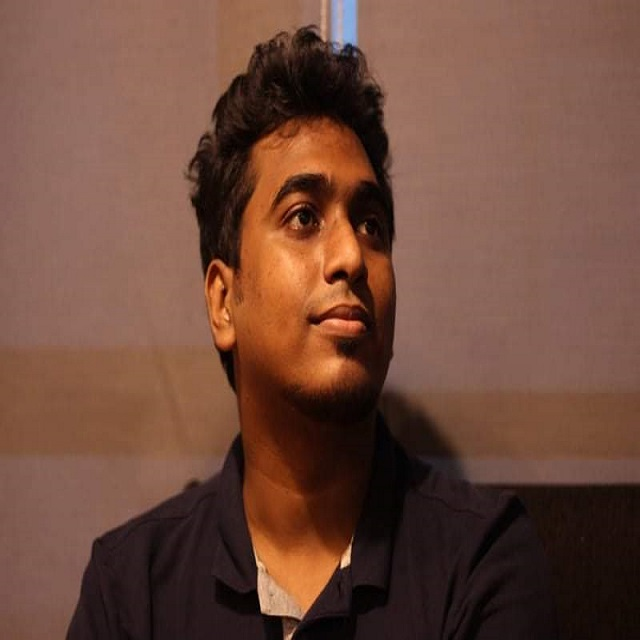
\includegraphics[trim= 0 0 0 0,clip,width=0.2\linewidth]{myfoto.jpeg}
	\hspace{8pt}
	\parbox[b]{5cm}{
	\metasection{Date of Birth:}{25 July, 1997}
	\metasection{Height:}{5'11"} 
	\metasection{Blood Type:}{B+}
	\metasection{Religion:}{Islam}	
	\metasection{Designation:}{Student \& Intern at ESRD,BUET}
	
	}
}

\end{center}
\end{minipage}}\\[-4pt]

%----------------------------------------------------------------------------------------
% EDUCATION
%----------------------------------------------------------------------------------------
\fcolorbox{light}{light}{
\begin{minipage}[c][0.2875\textheight][t]{\linewidth}
\vspace{1pt}
\hspace{26pt}
\parbox[c]{0.75\linewidth}{
%\cvsection{Education}

\cvevent{2014}{SSC}{}{Chittagong Collegiate School}{\: \: Group: Science}{ \: \: Grade: A+ (Golden)}

%\textcolor{softcol}{\hrule}

%
\cvevent{2016}{HSC}{}{Gov't Hazi Muhammad Mohsin College}{\: \: Group: Science}{ \: \: Grade: A+ (Golden)}

%\textcolor{softcol}{\hrule}

%
\cvevent{2017-Running}{BSC}{}{Bangladesh University of Engineering \& Technology}{\: \: Subject: Computer Science \& Engineering}{ \: \: Grade: Ongoing}

%\textcolor{softcol}{\hrule}

}
\hspace{18pt}
\textcolor{sectcol}{\rule[-3.2cm]{2pt}{7cm}}
\hspace{12pt}
\rotatebox[origin=c]{270}{\HUGE \textsc{Education}}
\end{minipage}}\\[-4pt]
%----------------------------------------------------------------------------------------
% EXPERIENCE
%----------------------------------------------------------------------------------------
\fcolorbox{white}{white}{
\begin{minipage}[c][0.36\textheight][t]{\linewidth}
\vspace{4pt}
\hspace{26pt}
\parbox[c]{0.75\linewidth}{
%
\cvevent{ }{Father}{ }{MD. Mizanur Rahman Khandaker}{\: \: Designation: Terminal Manager, Chittagong Port Authority}

%\textcolor{softcol}{\hrule}

%
\cvevent{ }{Mother}{ }{Nargis Akter}{\: \: Designation: Assistant Teacher, Dr. Khastagir Govt. Girl's High School}


%\textcolor{softcol}{\hrule}

%
\cvevent{ }{Sister}{ }{Nadia Mashiat}{\: \: Designation: Student, Institute of Educational Research, Chittagong University}

%\textcolor{softcol}{\hrule}

%
\cvevent{ }{Brother In Law}{ }{Asif Reza}{\: \: Designation: Assistant Director, Bangladesh Bank}{}



%\textcolor{softcol}{\hrule}


%

}
\hspace{18pt}
\textcolor{sectcol}{\rule[-3.2cm]{2pt}{7cm}}
\hspace{12pt}
\rotatebox[origin=c]{270}{\HUGE \textsc{Family Information}}
\end{minipage}}\\[-4pt]


%----------------------------------------------------------------------------------------
\fcolorbox{light}{light}{
	\begin{minipage}[c][0.36\textheight][t]{\linewidth}
		\vspace{4pt}
		\hspace{26pt}
		\parbox[c]{0.75\linewidth}{
			%\textcolor{softcol}{\hrule}
			
			\cvevent{ }{Paternal Uncle (Middle) }{ }{Kauser Khandaker}{\: \: Designation: Manager of Finance \& Operations at City of Wetaskiwin, Canada}
			%
			
			\cvevent{ }{Paternal Uncle (Younger) }{ }{Aman Khandaker}{\: \: Designation: Officer at CNF, Chittagong}
			
			%\textcolor{softcol}{\hrule}
			
			%
			\cvevent{ }{Maternal Uncle (Elder) }{ }{Babul Alam}{\: \: Designation: General Manager Incharge, Sonali Bank , Sylhet}
			
			
			%\textcolor{softcol}{\hrule}
			
			%
			\cvevent{ }{Maternal Uncle (Younger) }{ }{Mamunur Rashid}{\: \: Designation: Businessman, Shahrasti, Chandpur}
			
			
			%\textcolor{softcol}{\hrule}
			
			
			%
			
		}
		\hspace{18pt}
		\textcolor{sectcol}{\rule[-3.2cm]{2pt}{7cm}}
		\hspace{12pt}
		\rotatebox[origin=c]{270}{\HUGE \textsc{Family Information}}
\end{minipage}}\\[-4pt]
%---------------------------------------------------------------------
%----------------------------------------------------------------------------------------
\fcolorbox{white}{white}{
	\begin{minipage}[c][0.2875\textheight][t]{\linewidth}
		\vspace{1pt}
		\hspace{26pt}
		\parbox[c]{0.75\linewidth}{
			%\cvsection{Education}
			
			\cvevent{}{Current Address}{}{Flat No. F-11-4, VIP Tower, Kazir Dewri, Chittagong}
			
			%\textcolor{softcol}{\hrule}
			
			%
			\cvevent{}{Permanent Address}{}{House:Fakir Bari, Village:Sailcho, Thana:Barura, District:Comilla}
			
			%\textcolor{softcol}{\hrule}
			
			%
			\cvevent{}{Dhaka Address}{}{Room 203, Shere Bangla Hall BUET, Palashi, Dhaka}
			
			%\textcolor{softcol}{\hrule}
			
		}
		\hspace{18pt}
		\textcolor{sectcol}{\rule[-3.2cm]{2pt}{7cm}}
		\hspace{12pt}
		\rotatebox[origin=c]{270}{\HUGE \textsc{Address}}
\end{minipage}}\\[-4pt]
%----------------------------------------------------------------------------------------


%----------------------------------------------------------------------------------------
\fcolorbox{light}{light}{
	\begin{minipage}[c][0.2875\textheight][t]{\linewidth}
		\vspace{1pt}
		\hspace{26pt}
		\parbox[c]{0.75\linewidth}{
			%\cvsection{Education}
			
			\cvevent{}{Mobile No.}{}{Self: +8801521487070}{\: \: Parent: +8801838444486}
			
			%\textcolor{softcol}{\hrule}
			
			%
			\cvevent{}{Email}{}{minhaz725@gmail.com}
			
			%\textcolor{softcol}{\hrule}
			
			%
			\cvevent{}{Website}{}{https://www.minhazrahman.me}
			
			%\textcolor{softcol}{\hrule}
						
			
		}
		\hspace{18pt}
		\textcolor{sectcol}{\rule[-3.2cm]{2pt}{7cm}}
		\hspace{12pt}
		\rotatebox[origin=c]{270}{\HUGE \textsc{Contact Info}}
\end{minipage}}\\[-4pt]
%----------------------------------------------------------------------------------------


\end{document}
